\section{Systemmodelle}
% TODO T Nummern anpassen

\subsection{Objektmodelle}
% UML Klassendiagramme

\begin{figure}[H]
\centering
\includegraphics[scale=0.5]{../system_models/object_models/lambda_calculus.pdf}
\caption{UML Klassendiagramm zum Lambda-Kalkül}
\end{figure}

\subsection{Dynamische Modelle}
% UML Zustandsautomat, Sequenzdiagramm

%\newgeometry{left=40pt}
\begin{figure}[H]
\centering
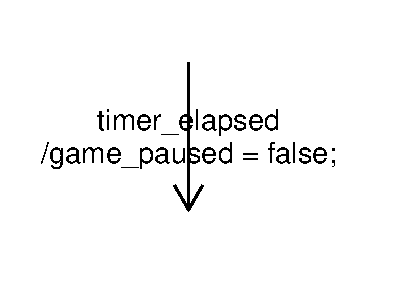
\includegraphics[scale=0.4]{../system_models/dynamic_models/menu_state_machine.pdf}
\caption{Zustandsautomat zur Menübedienung}
\end{figure}
%\restoregeometry

\begin{figure}[H]
\centering
\includegraphics[scale=0.55]{../system_models/dynamic_models/game_level_state_machine.pdf}
\caption{Zustandsautomat zum Ablauf eines Levels}
\end{figure}

\begin{figure}[H]
\centering
\includegraphics[scale=0.55]{../system_models/dynamic_models/reduction_mode_state_machine.pdf}
\caption{Zustandsautomat zur Funktion des Reduktions-Modus}
\end{figure}

%GUI

\subsection{Benutzerschnittstelle}
%../GUI-Entwurf/_jpeg_numeration/registration1.gpej
%1-pflichtenheft/
\newcounter{B.SS}
\begin{figure}[H]

\centering
\refstepcounter{B.SS}\label{fig:Sprachauswahl}
\includegraphics[scale=0.55]{../gui/_jpeg_numeration/registration1.jpg}

\caption{Sprachauswahl}


\end{figure}

\begin{figure}[H]
\centering
\refstepcounter{B.SS}\label{fig:Namenseingabe} 
\includegraphics[scale=0.55]
{../gui/_jpeg_numeration/registration2.jpg}
\caption{Namenseingabe}
\end{figure}

\begin{figure}[H]
\centering
\refstepcounter{B.SS}\label{fig:Avatarauswahl}
\includegraphics[scale=0.55]{../gui/_jpeg_numeration/registration3.jpg}
\caption{Avatarauswahl}
\end{figure}

\begin{figure}[H]
\centering
\refstepcounter{B.SS}\label{fig:Profilauswahl}
\includegraphics[scale=0.55]{../gui/_jpeg_numeration/choose_profile.jpg}
\caption{Profilauswahl}
\end{figure}

\begin{figure}[H]
\centering
\refstepcounter{B.SS}\label{fig:Welcome}
\includegraphics[scale=0.55]{../gui/_jpeg_numeration/welcome.jpg}
\caption{Begrüssungsbildschirm}
\end{figure}

\begin{figure}[H]
\centering
\refstepcounter{B.SS}\label{fig:Hauptmenu}
\includegraphics[scale=0.55]{../gui/_jpeg_numeration/main_manu.jpg}
\caption{Hauptmenu}
\end{figure}

\begin{figure}[H]
\centering
\refstepcounter{B.SS}\label{fig:Einstellungen}
\includegraphics[scale=0.55]{../gui/_jpeg_numeration/settings.jpg}
\caption{Einstellungen}
\end{figure}

\begin{figure}[H]
\centering
\refstepcounter{B.SS}\label{fig:Statistik}
\includegraphics[scale=0.55]{../gui/_jpeg_numeration/stat.jpg}
\caption{Statistik}
\end{figure}

\begin{figure}[H]
\centering
\refstepcounter{B.SS}\label{fig:game}
\includegraphics[scale=0.55]{../gui/_jpeg_numeration/game.jpg}
\caption{Editormodus}
\end{figure}

\begin{figure}[H]
\centering
\refstepcounter{B.SS}\label{fig:game_paused}
\includegraphics[scale=0.55]{../gui/_jpeg_numeration/game_paused.jpg}
\caption{Editormodus pausiert}
\end{figure}

\begin{figure}[H]
\centering
\refstepcounter{B.SS}\label{fig:game_teachermode}
\includegraphics[scale=0.55]{../gui/_jpeg_numeration/game_teachermode.jpg}
\caption{Editormodus mit eingeschaltetem Lehrermodus}
\end{figure}

\begin{figure}[H]
\centering
\refstepcounter{B.SS}\label{fig:game_play_started}
\includegraphics[scale=0.55]{../gui/_jpeg_numeration/game_play_started.jpg}
\caption{Reduktionsmodus}
\end{figure}

\begin{figure}[H]
\centering
\refstepcounter{B.SS}\label{fig:game_completed}
\includegraphics[scale=0.55]{../gui/_jpeg_numeration/game_completed.jpg}
\caption{Levelabschluss}
\end{figure}

\begin{figure}[H]
\centering
\refstepcounter{B.SS}\label{fig:game_freemode}
\includegraphics[scale=0.55]{../gui/_jpeg_numeration/game_freemode.jpg}
\caption{Freier Editormodus}
\end{figure}

\begin{figure}[H]
\centering
\refstepcounter{B.SS}\label{fig:achievments}
\includegraphics[scale=0.55]{../gui/_jpeg_numeration/achievements.jpg}
\caption{Achievements}
\end{figure}

\begin{figure}[H]
\centering
\refstepcounter{B.SS}\label{fig:level}
\includegraphics[scale=0.55]{../gui/_jpeg_numeration/level.jpg}
\caption{Levels}
\end{figure}

\begin{figure}[H]
\refstepcounter{B.SS}\label{fig:shop}
\centering
\includegraphics[scale=0.55]{../gui/_jpeg_numeration/shop.jpg}
\caption{Shop}
\end{figure}

\begin{figure}[H]
\refstepcounter{B.SS}\label{fig:shop_popup}
\centering
\includegraphics[scale=0.55]{../gui/_jpeg_numeration/shop_popup.jpg}
\caption{shoppopup}
\end{figure}

